\documentclass[a4paper,12pt]{article}

\usepackage{graphicx} % Required for inserting images
\usepackage{amsmath,amssymb,amsfonts}
\usepackage{subcaption}
% -----------------------
% Package Imports
% -----------------------

% Set page margins
\usepackage[a4paper, top=1in, bottom=0.8in, left=1.1in, right=0.8in]{geometry}

% Use Times New Roman font
\usepackage{times}

% Add page numbering
\pagestyle{plain}
\usepackage{multirow}
% Enable graphics inclusion
\usepackage{graphicx}
\usepackage{float}
% Enable code listings
\usepackage{listings}
\usepackage{xcolor} % For customizing code colors

% Define MATLAB style for listings
\lstdefinestyle{vscode-light}{
	language=Matlab,
	basicstyle=\ttfamily\footnotesize,
	keywordstyle=\color{blue},
	commentstyle=\color{gray},
	stringstyle=\color{red},
	numberstyle=\tiny\color{black},
	numbersep=5pt,
	frame=single,
	backgroundcolor=\color{gray!10},
	breaklines=true,
	captionpos=b,
	tabsize=4,
	showstringspaces=false,
	numbers=left,  % Enable line numbering on the left
	stepnumber=1,  % Line numbers increment by 1
	numberfirstline=true, % Number the first line
}
\setlength{\parindent}{0pt}
\begin{document}
	\section{Experiment No. 2}
	
	\section{Experiment Title }
	Observation of no load magnetization curve of separately excited DC generator.
	\section{Objective}
	
	The objectives of this lab are as follows:
	
	\begin{itemize}
		\item To study the relationship between field current ($I_f$) and induced voltage ($E_g$) in a DC generator.
		\item To observe the hysteresis loop in a DC generator by increasing and then decreasing the field current.
		\item To analyze the impact of residual magnetism and retentivity on the generator's performance.
		\item To evaluate how changes in speed affect the induced voltage in a DC generator.
	\end{itemize}
	\section{Theory}
	
	The induced voltage in a DC generator is dependent on the magnetic flux and the speed of the machine, assuming other factors are constant. If the speed of the driving mechanism remains constant and the flux in the generator is varied, the induced voltage will change accordingly. Initially, when there is no current in the field coils, there is still a small flux due to residual magnetism in the field poles, resulting in a small induced voltage (Point 1). 
	
	As the current in the field coils increases, the flux also increases, leading to a rise in the induced voltage.
	
	\begin{figure}[H]
		\centering
		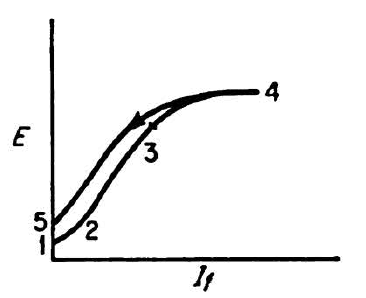
\includegraphics[width=0.4\linewidth]{Images/1} % Correct the folder path for the image
		\caption{Induced voltage vs. Field current characteristic curve}
		\label{fig:1}
	\end{figure}
	
	From Figure \ref{fig:1}, it can be observed that the induced voltage increases proportionally with the field current up to a certain point (Points 2 to 3). Beyond Point 3, further increases in the field current result in smaller increments in the induced voltage (Points 3 to 4). This behavior is due to the magnetic saturation of the circuit. In any magnetic circuit, increasing the magneto-motive force (MMF) increases the magnetic flux until saturation is reached. Beyond this point, further increases in MMF result in only slight increases in flux. Since the induced voltage is directly related to the magnetic flux, the voltage increase also diminishes after saturation.
	
	If the field current is now reduced, the decreasing voltage does not follow the same path as during the increase. Instead, the voltage decreases from Point 4 to Point 5, forming a hysteresis loop. This phenomenon occurs due to the retentivity of the magnetic material in the circuit. When measuring the magnetization curve in a laboratory setting, it is important to continuously increase the field current until the maximum value is reached. After that, the current should only be decreased until it reaches zero. Fluctuating the current back and forth in an attempt to achieve specific values can result in smaller hysteresis loops and inconsistent results.
	
	Another challenge in measuring the magnetization curve is maintaining a constant speed. Since the induced voltage depends on both the flux and the speed of the machine, any speed variation will lead to corresponding variations in voltage. However, this issue can be mitigated by calculating the voltage at the desired speed, given the induced voltage at a different speed.
	\section{Required Apparatus:}
	\begin{enumerate}
	\item Variable DC Supply (Ratings: Voltage: 0-500V, Current: 4A),	
	\item Three Phase Power Supply (Ratings: Voltage: 400V, Current: 10A),	
	\item DC Multimeter (Ratings: Voltage: 600V, Current: 20A) 
	\item Three Phase Asynchronous Motor (Ratings: Power: 500W, Voltage: 400V/230V, Current: 1.8A/1.3A, Speed: 1380 rpm),
	\item DC Generator (Ratings: Power: 300W, Voltage: 220V, Current: 1.4A)
	\item Tacho-Generator (Ratings: Current: 0.07A max, Speed: 5000 rpm max).
	\end{enumerate}
	\section{Circuit Diagram:}
		\begin{figure}[H]
		\centering
		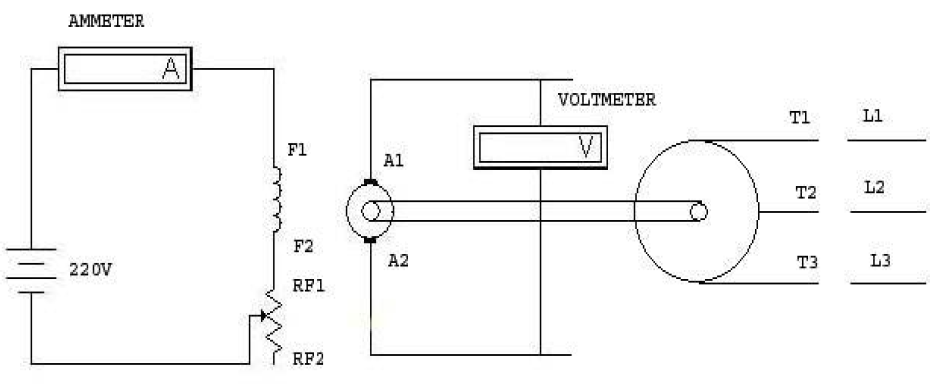
\includegraphics[width=0.9\linewidth]{Images/2} % Correct the folder path for the image
		\caption{Circuit Diagram of the experiment}
		\label{fig:2}
	\end{figure}
	\section{Data Table:}
\begin{table}[H]
	\centering
	\caption{Readings of Field Current and Induced EMF for Decreasing Current}
\scalebox{1}{
	
	\begin{tabular}{|c|cc|cc|}
		\hline
		\multicolumn{1}{|l|}{\textbf{SI No.}} & \multicolumn{2}{c|}{\textbf{Increasing Current}}                                                                                                                                        & \multicolumn{2}{c|}{\textbf{Decreasing Current}}                                                                                                                                \\ \hline
		& \multicolumn{1}{c|}{\textbf{\begin{tabular}[c]{@{}c@{}}Field Current\\         $I_{f_i}$ \\(A)\end{tabular}}} & \textbf{\begin{tabular}[c]{@{}c@{}}Induced Voltage\\ $E_{g_i}$\\(V)\end{tabular}} & \multicolumn{1}{l|}{\textbf{\begin{tabular}[c]{@{}c@{}}Field Current \\ $I_{f_d}$\\(A)\end{tabular}}} & \textbf{\begin{tabular}[c]{@{}c@{}}Induced voltage\\ $E_{g_d}$\\(V)\end{tabular}} \\ \cline{2-5} 
		1.                                    & \multicolumn{1}{c|}{0.00}                                                                                & 63.48                                                                        & \multicolumn{1}{c|}{0.11}                                                                        & 211.87                                                                       \\ \hline
		2.                                    & \multicolumn{1}{c|}{0.015}                                                                               & 78.12                                                                        & \multicolumn{1}{c|}{0.092}                                                                       & 208.31                                                                       \\ \hline
		3.                                    & \multicolumn{1}{c|}{0.021}                                                                               & 93.63                                                                        & \multicolumn{1}{c|}{0.084}                                                                       & 199.83                                                                       \\ \hline
		4.                                    & \multicolumn{1}{c|}{0.025}                                                                               & 109.25                                                                       & \multicolumn{1}{c|}{0.065}                                                                       & 189.09                                                                       \\ \hline
		5.                                    & \multicolumn{1}{c|}{0.030}                                                                               & 120.4                                                                        & \multicolumn{1}{c|}{0.060}                                                                       & 184.5                                                                        \\ \hline
		6.                                    & \multicolumn{1}{c|}{0.036}                                                                               & 126.14                                                                       & \multicolumn{1}{c|}{0.057}                                                                       & 179.35                                                                       \\ \hline
		7.                                    & \multicolumn{1}{c|}{0.048}                                                                               & 149.88                                                                       & \multicolumn{1}{c|}{0.046}                                                                       & 161.97                                                                       \\ \hline
		8.                                    & \multicolumn{1}{c|}{0.055}                                                                               & 172..26                                                                      & \multicolumn{1}{c|}{0.039}                                                                       & 139.23                                                                       \\ \hline
		9.                                    & \multicolumn{1}{c|}{0.067}                                                                               & 186.00                                                                       & \multicolumn{1}{c|}{0.026}                                                                       & 120.34                                                                       \\ \hline
		10.                                   & \multicolumn{1}{c|}{0.082}                                                                               & 192.74                                                                       & \multicolumn{1}{c|}{0.020}                                                                       & 103.72                                                                       \\ \hline
		11.                                   & \multicolumn{1}{c|}{0.096}                                                                               & 206.22                                                                       & \multicolumn{1}{c|}{0.016}                                                                       & 89.21                                                                        \\ \hline
		12.                                   & \multicolumn{1}{c|}{0.110}                                                                               & 211.87                                                                       & \multicolumn{1}{c|}{0.00}                                                                        & 70.57                                                                        \\ \hline
	\end{tabular}}
\end{table}

\section{Graph:}
\begin{figure}[H]
	\centering
	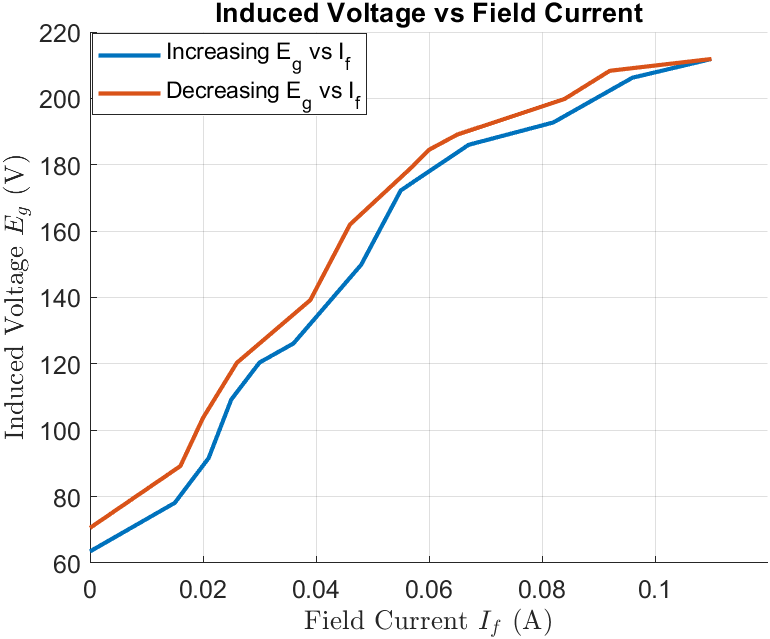
\includegraphics[width=0.8\linewidth]{Images/3.3}
	\caption{Induced voltage ($E_g$) vs. Field current ($I_f$) characteristic curve}
	\label{fig:3}
\end{figure}
\newpage
\subsection{Matlab Code:}

\begin{lstlisting}[style=vscode-light, caption={MATLAB code for plotting data}]
  % Given data
  inc_field_current = [0.00, 0.015, 0.021, 0.025, 0.030, 0.036, 0.048, 0.055, 0.067, 0.082, 0.096, 0.11];
  dec_field_current1 = [0.11, 0.092, 0.084, 0.065, 0.060, 0.057, 0.046, 0.039, 0.026, 0.020, 0.016, 0.00];
  
  inc_generated_voltage = [63.48, 78.12, 91.63, 109.25, 120.4, 126.14, 149.88, 172.26, 186, 192.74, 206.22, 211.87];
  dec_generated_voltage1 = [211.87, 208.31, 199.83, 189.09, 184.5, 179.35, 161.97, 139.23, 120.34, 103.72, 89.21, 70.57];
  % Plot the data
  figure;
  hold on;
  plot(inc_field_current, inc_generated_voltage,'DisplayName', 'Increasing E_g vs I_f ', 'LineWidth', 2);
  plot(dec_field_current1, dec_generated_voltage1,'DisplayName', 'Decreasing E_g vs I_f', 'LineWidth', 2);
  % Add labels,title,grid and legend 
  xlabel('Field Current $I_f$ (A)', 'Interpreter', 'latex', 'FontSize', 12);
  ylabel('Induced Voltage $E_g$ (V)', 'Interpreter', 'latex', 'FontSize', 12);
  title('Induced Voltage vs Field Current', 'FontSize', 16);
  grid on;
  legend('show', 'Location', 'Best');
  set(gca, 'FontSize', 12);
  hold off;
  
\end{lstlisting}

\section{Discussion}

This experiment examined the relationship between field current ($I_f$) and induced voltage ($E_g$) in a DC generator. The results show a nonlinear relationship, with induced voltage increasing proportionally at first and then more slowly due to magnetic saturation. The hysteresis effect was also observed, as the voltage did not follow the same path when decreasing the field current, highlighting the influence of residual magnetism.\\

Minor speed variations may have affected the induced voltage, but these were kept minimal. Overall, the results align with theoretical expectations, though improvements in measurement accuracy and speed control could enhance the precision of the experiment.\\

Overall, the results align well with theoretical expectations of magnetic saturation and hysteresis. However, the precision of the experiment could be improved by using more accurate control of the generator speed and by using a higher resolution for current and voltage measurements. 


\end{document}